%%%%%%%% ICML 2020 EXAMPLE LATEX SUBMISSION FILE %%%%%%%%%%%%%%%%%

\documentclass{article}

\usepackage{microtype}
\usepackage{graphicx}
\usepackage{subcaption}
\usepackage{booktabs}
\usepackage{amsmath}
\usepackage{placeins}

% hyperref makes hyperlinks in the resulting PDF.
% If your build breaks (sometimes temporarily if a hyperlink spans a page)
% please comment out the following usepackage line and replace
% \usepackage{icml2020} with \usepackage[nohyperref]{icml2020} above.
\usepackage{hyperref}

% Attempt to make hyperref and algorithmic work together better:
\newcommand{\theHalgorithm}{\arabic{algorithm}}

% Use the following line for the initial blind version submitted for review:
\usepackage{icml2020}
% \pagestyle{plain} 

% If accepted, instead use the following line for the camera-ready submission:
%\usepackage[accepted]{icml2020}

% The \icmltitle you define below is probably too long as a header.
% Therefore, a short form for the running title is supplied here:.

% Informative title – Please create an informative title for your term paper that is relevant to the content of the paper. It can be a longer title (roughly 5-10 words). You can think of it as an abstract of the abstract. It should not be generic like “Course term paper” or “Project paper”.

\newcommand{\papertitle}{Twin-Delayed Deep Deterministic Policy Gradient (TD3): \\ A Reimplementation and Discussion for ECE 570}
\icmltitlerunning{Twin-Delayed Deep Deterministic Policy Gradient (TD3)}

\begin{document}

\twocolumn[

\icmltitle{\papertitle}
\icmlsetsymbol{equal}{*}

\begin{icmlauthorlist}
\icmlauthor{Nicholas B. LaFarge}{equal,pu}
\end{icmlauthorlist}

\icmlaffiliation{pu}{Department of Aeronautics and Astronautics, Purdue University, West Lafayette, IN, USA}
\icmlcorrespondingauthor{Nicholas B. LaFarge}{nlafarge@purdue.edu}
\icmlkeywords{Machine Learning, TD3, RL, ICML}
\vskip 0.3in
]
\printAffiliationsAndNotice{\icmlEqualContribution}
\newcommand{\note}[1]{{\color{red}\textit{#1}}}


\begin{abstract}
Many recent advancements in reinforcement learning for continuous controls tasks involve on-policy training. In this paradigm, data must be sampled from the most recent policy, and immediately discarded after optimization. The constant need for new environmental interactions renders these approaches extremely data inefficient and sensitive to hyper-parameter tuning values. Given these limitations, several authors have attempted to construct off-policy training schemes that do not suffer from the same inconsistencies apparent in previous work. The successful construction of off-policy training methods by \cite{td3}, \cite{sac}, and \cite{ofir} achieve remarkable state-of-the-art results, vastly outperforming their on-policy counterparts. This investigation seeks to reproduce the learning approach presented by  \cite{td3}, and to compare learning results with an alternative algorithm.
\end{abstract}



% Approximately two to three pages of this paper should be a substantive critique of the three (or more) papers that you have read.
\section{Previous Work}

Combining function approximation, large continuous action spaces, and off-policy training is a historically challenging combination for Reinforcement Learning (RL) algorithms. Each investigation reviewed in this research effort presents a novel approach that enables off-policy training in historically challenging domains. Many current state-of-the-art approaches prior to the papers reviewed here, such as the well-known Proximal Policy Optimization (PPO) algorithm \citep{ppo}, require that all training data be collected under the current policy (i.e. ``on-policy''). This is extremely limiting for data efficiency because as soon as the neural network performs its optimization steps, all prior data must be discarded. In contrast, off-policy approaches retain past data, enabling faster learning with fewer environmental interactions. While off-policy approaches are attractive, they are historically inflexible to hyper-parameter tuning, and often unstable for learning. The overall thread that connects these three papers is they each improve state-of-the-art on-policy RL results by finding different ways to stabilize off-policy learning for continuous control tasks.

\subsection{Paper 1: Addressing Function Approximation Error in Actor-Critic Methods \citep{td3}}
Fujimoto et al. propose improvements to the well-known deep RL algorithm ``Deep Deterministic Policy Gradient'' (DDPG), originally detailed by \citep{ddpg}. DDPG achieved promising results, but suffered from inconsitency in training. The improvements to DDPG suggested by Fujimoto et al. create a new approach that is interchangeably referred to as either ``Twin-Delayed Deep Deterministic Policy Gradient'', ``Twin-Delayed DDPG'', or most concisely, TD3. While TD3 is directly built off DDPG, the emergence of the TD3 algorithm can be directly traced back to early RL contributions through a series of major landmark advancements in RL.  

Various RL approaches use the state-action value function $Q(s,a)$,  updated by iterating on the Bellman equation, to formulate an effective policy for off-policy control. The $Q(s,a)$ function can be easily understood as the value of taking a particular action $a$ given a state or observation $s$. For example, in the game of tic-tac-toe, the state denotes the current board configuration, and the action involves choosing a square and drawing `X' or `O'. Hence, a high value for $Q$ might correspond to a winning tic-tac-toe move, and a low value for $Q$ could be an action that leaves a winning move open for the opponent. An early breakthrough for problems with discrete state and action spaces occurred in 1989 with \textit{Q-Learning}: a temporal difference learning algorithm that allows powerful agents to be trained in an off-policy manor (recall that ``off-policy'' indicates that data may be collected from any policy, not necessarily from the agent being optimized) \citep{textbook}. While effective, this approach, along with other RL approaches at the time, was limited by the assumption of discrete spaces due to the lack of effective nonlinear function approximators. A major breakthrough in RL came in 2015 when the $Q$-Learning algorithm was extended to continuous state space problems with the Deep $Q$-Network (DQN) algorithm \citep{dqn}. The DQN approach involves the same update rule as $Q$-Learning, but rather than direct computation, is able to effectively estimate the $Q$ function using a neural network: alleviating the need for tabulated results. However, similar to $Q$-Learning, DQN still suffered from the discrete action space assumption. This was okay for Atari game tasks, where actions were limited to available Atari controls, but limited the applicability for continuous control tasks, such as robotics. Addressing this limitation, \citep{ddpg} introduced Deep Deterministic Policy Gradient (DDPG): an extension of DQN that uses a second ``actor'' neural network to construct a parameterized action function, and performed the $Q(s,a)$ update with the new actor network. A key portion of DDPG is the inclusion of ``target'' networks for both the actor and value (i.e. \textit{critic}) networks (a similar target approach is also seen in the double DQN extension of the DQN approach). By including duplicate networks, the second ``target'' networks may be held constant while the actual networks are updated. This is a more stable process because it doesn't involve continuously updating estimates to be used in the minibatch updates. While powerful, however, DDPG contained several notable limitation. In particular, the value function is often over-estimated, which leads to a significant bias in learning.

Twin-Delated DDPG (TD3) addresses the instability of DDPG in several ways. First, two separate value networks are included. Taking the minimum value estimate of the two networks mitigates the effect of the value function over-estimation bias present in DDPG (along with other actor-critic schemes). Next, DDPG involves \textit{bootstrapping}, i.e., performing updates based on estimates rather than true values. Noisy estimates cause noisy gradients which pose significant difficulty in network optimization. \cite{td3} seek to mitigate this error by delaying updates to the actor network in hopes that additional updates to the critic network will provide more accurate estimates for the actor updates. Finally, to avoid peak overfitting in the policy network, policy smoothing is included, which introduces a small amount of clipped random noise to the output of the target policy. Together, these improvements form the TD3 variant of DDPG.

Fujimoto et. al. provide an extremely practical and concise account of their algorithm, contributions, and overall approach. Results from experiments are very compelling: outperforming state-of-the-art algorithms in virtually every task (including their improved version of DDPG). While I understand this is not possible for a conference paper with length limitations, one drawback of this paper is that I don't think it would really be possible to fully understand the algorithm from this paper as a standalone document. In particular, understanding DDPG is vital to understanding TD3's improvements. In turn, a thorough understanding DDPG requires knowing the DQN algorithm, which itself builds off a base-knowledge of Q-Learning. I saw these as the most important `steps' leading up to TD3, but this is by no means an exhaustive literature background for the TD3 approach. While this necessitated a significant amount of additional reading to fully grasp the approach, I don't fault the authors because they had a very helpful ``Related Work'' section that directed me to various sources to understand more of the underlying theory that enables their approach.

Literature review aside, there are several additional specific points worth mentioning. First, the authors did an excellent job in their discussion of the overestimation bias of value functions in actor-critic approaches. In addition to a theoretical understanding, the numerical results enhanced the discussion, and made it easily understandable for the reader. If I had to single out one part that could perhaps be clarified, it would be the section on smoothing regularization. I understand how the noise helps negate negative effects of peaks in the value estimate, however I don't think it is very clear how this noise should be produced, what scale it should be, and why it must come from a normal distribution. The appendices address how the policy must be clipped to avoid impossible actions from the noise, but I think a more thorough theoretical analysis of the underlying statistics could reveal a more rigorous way to choose the random process. One final concern I have about the approach itself is the overall complexity. Although results demonstrate its performance, the complexity of having six total neural networks (DQN originally only had one!) indicates to me that there may be unintended consequences of these complex interactions.

\subsection{Paper 2: Soft Actor-Critic: Off-Policy Maximum Entropy Deep Reinforcement Learning with a Stochastic Actor\citep{sac}}
Both \citep{td3} and \citep{sac} concurrently propose novel RL approaches that involve off-policy training. While their approaches differ, their goal is the same: to improve the sample efficiency of continuous control reinforcement learning tasks by allowing networks to be trained in an off-policy manor. An additional limitation to many current methods (on-policy and off-policy) is their sensitivity to hyper-parameter tuning. Training is computationally expensive, and it is difficult to determine a set of hyper-parameters that works on a wide range of problems. \cite{sac} seek to address these to limitations through a novel approach called Soft Actor-Critic (SAC). Published concurrently with TD3, both methods are able to overcome training instability in off-policy methods, and address the two aforementioned key motivations, i.e., hyper-parameter sensitivity and sample efficiency. 

The main contribution of SAC that differentiates it from TD3 is the inclusion of an entropy regularization term in the objective functions. Typical RL methods seek to maximize the expected future discounted return, i.e., the discounted sum of future rewards. Soft Actor-Critic augments this traditional reward function with the inclusion of an expected entropy term. By maximizing entropy as well, the optimizer seeks to maximize the expected returns while acting as diversely as possible. This is related to another classical RL concept: the balance between exploration and exploitation. By maximizing entropy, the algorithm is encouraged to explore the action space much more thoroughly, which increases the chances of converging on an effective policy, rather than a local minimum. One final notable difference between SAC and TD3 is that SAC trains a stochastic policy (like PPO \citep{ppo}), and hence does not need the policy smoothing step described in the TD3 section.

One of the most striking portions of this paper is the abundant theoretical justification provided for their entropy regularization approach and soft policy iteration learning scheme. It is very common in machine learning to have impressive results that rely on some heuristic. While still effective, knowing \textit{why} something works provides much opportunities for analyitical analysis and potential future improvements. The authors' derivation of soft policy iteration provides a solid foundation for their approach. I also thought it was interesting how the authors specified which types of continuous controls tasks we may expect to see SAC perform the best (compared to other methods). In particular, tasks with large action spaces benefit the most from the increased exploration enabled by the entropy term in the cost function. This is demonstrated through the Humanoid (rllab) simulation, where the comparative algorithms are all dramatically sub-optimal compared to the SAC results.

\subsection{Paper 3: Data-Efficient Hierarchical Reinforcement Learning \citep{ofir}}
Like the previous two papers, \citep{ofir} also look to improve on current methodologies that rely on off-policy data. However, in contrast to \cite{sac} and \cite{td3},  Nachum et al. propose an approach to \textit{Hierarchical reinforcement learning (HRL)}. Hierarchical RL refers to decomposed problems divided into parent and child tasks, rather than relying on one RL algorithm to address all tasks involved in a problem. As an intuitive example, a robotic problem might involve a parent process (the robot performing some task), and a child task (learning how to manipulate the low-level robotics to move arms, legs, etc.). \citep{ofir} propose \textit{HIRO}: a more flexible, general, off-policy approach to HRL with better data efficiency than prior work. Notable in the context of this investigation, \citep{ofir} choose TD3 \cite{td3} as their temporal difference learning algorithm for subtasks.

There are several key contributions that aid in the success of \textit{HIRO}. The first is in the interaction between the high and low level policies. \citep{ofir} formulate the reward mechanism for the lower-level policy to match desired observations via low-level actions. This is simpler and more general than prior methods since the observation signal is directly employed, rather than relying on an embedded space. Next, and perhaps most importantly, is the application of an off-policy RL learning approach. To address prior instability in applying off-policy algorithms to HRL tasks, \citep{ofir} propose a correction to alter past experience to include actions that maximize probability of a particular past action occurring. This corrections process is needed because the relationship between past high/low level processes is fundamentally different than future ones. Without employing the proposed correction, optimization steps are included that involve high/low level interactions that would not occur, and are therefore not helpful to the training process. These key contributions allow \textit{HIRO} to be trained in a much more data-efficient manor, and produce state-of-the-art results in sample hierarchical navigation tasks.

One weakness of this paper I thought was their discussion of the hierarchical subdivisions of the RL process. While their practical examples gave a very intuitive understanding of the approach, some of the theoretical discussion of the hierarchy was more difficult to follow. For example, I thought the diagram in Figure 2 of \citep{ofir} was an over-complicated way to express the interaction between the high and low level policies. That said, the authors did a good job providing sufficient detail to replicate experiments, with a good mix of theoretical justification and numerical results. In particular, since their key contribution for enabling off-policy RL involved the labeling corrections process, I found the numerical experiments involving correction variants to be particularly persuasive, which gave me confidence that their corrections approach is viable for these challenging problems.





% Approximately three to four pages of this paper should be a description of your implementation, evaluation and discussion of the method from at least one of the papers.
\section{Simulation Results}

This investigation involves reimplementing the TD3 and DDPG algorithms, and testing them on various tasks. DDPG results are presented alongside TD3 to demonstrate their relative performance, however the reimplementation of TD3 remains the fundamental goal of this project, and therefore discussion is focused on TD3 in particular. Details regarding the reimplementation effort are presented in Section \ref{sec:implementation}, followed by and evaluation and discussion of the TD3 algorithm in Section \ref{sec:eval}. 

\subsection{Implementation Details} \label{sec:implementation}

Numerous high-quality baseline implementations are available online for TD3, including the one available directly from the authors. For this research effort, I chose to reimplement the Tensorflow version included in the OpenAI ``Spinning Up'' series \cite{SpinningUp2018}. Spinning Up is an educational tool produced by OpenAI that provides well-documented baseline versions of major RL algorithms, without the added complexity of other comparable baselines (included the ``baselines'' versions written by OpenAI). Their simplicity is indented to make the algorithms more approachable for newer researchers wanting to understand the approaches. I chose to reimplement the Spinning Up version over the one provided by \cite{td3} simply to gain more exposure to Tensorflow as opposed to PyTorch. Furthermore, recall that TD3 is an improved version of DDPG. To evaluate this improvement, I also implemented Spinning Up's DDPG code. This provided both a benchmark for running experiments, as well as illuminating the code details for where TD3 stands apart from DDPG.

The implementation included in this research project differs its from original Spinning Up source \cite{SpinningUp2018} in several notable ways. First, the original implementation defines the model, learning algorithm, and running script all in one place. In this paradigm, each new learning algorithm must re-implement the runner script (i.e. the basic script that keeps track of agent-environment interaction and stores relevant values). For increased flexibility, I chose to decouple these three parts into their own distinct sections of code. Furthermore, their implementation is based on tensorflow 1, and I added some modifications to allow the code to run using tensorflow 2.

First, in my version, the models are defined explicitly in their own classes in an object-oriented manor. The original implementation included duplicate code for defining models, and used a multi-layer perceptron function that made it difficult at times to keep track of the network details. While their way is likely more flexible, explicitly defining models was useful for this investigation because it simplified the process and made the code more easily understandable. Actor and critic networks are implemented as fully-connected feedforward networks, and the architectures are given in Table \ref{tab:actor} and \ref{tab:critic} for the actor and critic networks, respectively.

\begin{table}[!h]
\centering
\caption{TD3 Actor Architecture}
\begin{tabular}{|p{0.5cm}|p{2.cm}|p{1.5cm}|p{1.5cm}|}
\hline
\# & Input Size & Units & Activation \\
\hline
1 & state & 256 & ReLU\\
2 & 256 & 256 & ReLU\\
3 & 256 & action & Tanh\\
\hline
\end{tabular}
\label{tab:actor}
\end{table}
Next, I took a completely different approach for the runner script, and did not use their runner code as a source for mine. I separated my runner out in its own file such that the DDPG and TD3 agents could be easily interchanged, and all running code exists in one common place. This is very different than the original version where each algorithm has its own running mechanism. In implementing a new runner, one important difference between the original and reimplemented versions are that training is now conducted based on episodes, whereas in the original source, the learning process entirely formulated around a running counter of agent-environment interactions, and episodes are not at the forefront of the runner script. Finally, the overall learning is reorganized in my version to facilitate interaction with the model and runner scripts, and to increase code readability. I implemented my own methods for storing data as learning progresses. Mine is much simpler, and lacks much of the power (and complexity) of the original data storage method.

\begin{table}[!h]
\centering
\caption{TD3 Critic Architecture}
\begin{tabular}{|p{0.5cm}|p{2.cm}|p{1.5cm}|p{1.5cm}|}
\hline
\# & Input Size & Units & Activation \\
\hline
1 & state, action & 256 & ReLU\\
2 & 256 & 256 & ReLU\\
3 & 256 & 1 & Linear\\
\hline
\end{tabular}
\label{tab:critic}
\end{table}

Finally, two additional minor changes are worth noting. First, I changed how the networks are saved and loaded, and added the ability to load the network at a particular save point (to evaluate how learning occurs over time). Next, the most difficult aspect of the implementation for me to understand was how the action gradients were computed. While the original Spinning Up source uses a tensorflow trick to compute the gradients (and avoid updating other networks at the same time), I came across other implementations \footnote{The alternate form of this update is based on implementations by \href{https://github.com/google-research}{Google Research} and \href{https://github.com/tensorlayer/tensorlayer/}{TensorLayer}.} that computed these action gradients directly. I included the code to perform this step in both ways to verify that my implementation of this key point functions properly.


\subsubsection{hyper-parameters}\label{sec:hyperparams}

\begin{figure*}[!th]
\centering
  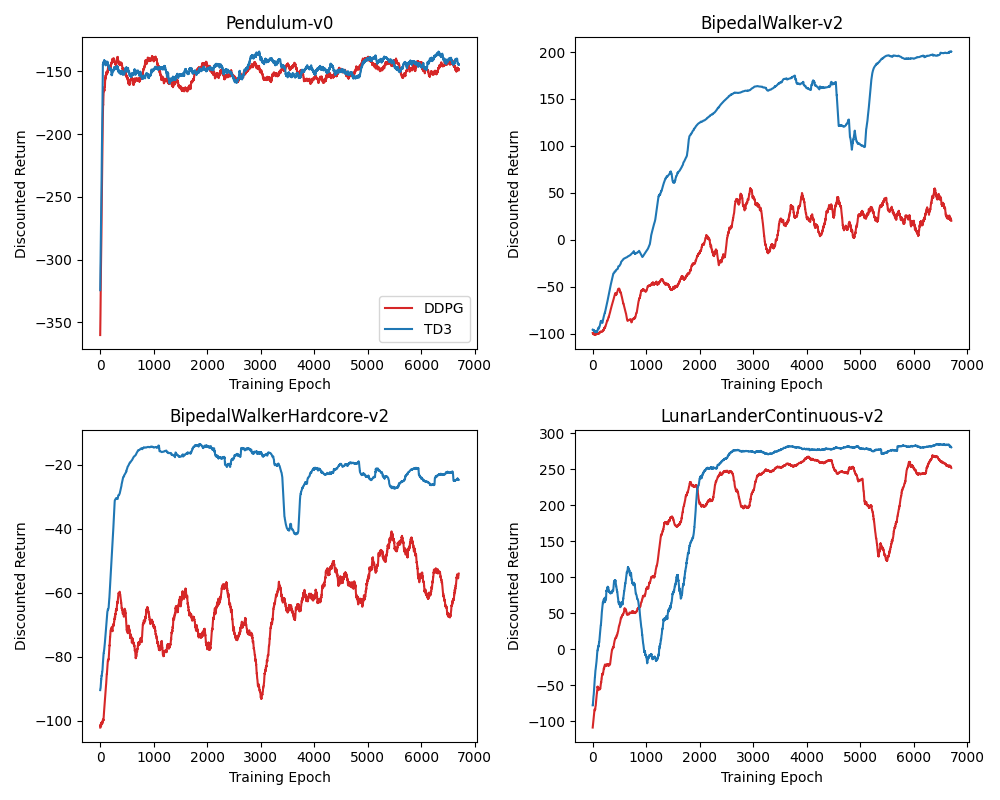
\includegraphics[scale=0.5]{figures/td3_vs_ddpg}
  \caption{Reward moving average of DDPG (red) vs TD3 (blue) across four sample OpenAI environments. TD3 reaches a more optimal solution than DDPG in three of four environments, and is comparable to DDPG in the simplest example (Pendulum-v0). However, despite performing better than DDPG on BipedalWalkerHardcore-v2, neither policy is able to solve the given problem.}
  \label{fig:td3_vs_ddpg}
\end{figure*}
Compared to some other RL approaches, TD3 is somewhat flexible for hyper-parameter selection. While experiment results could very likely be improved with task-specific hyper-parameter tuning, time and computational limitations made that challenging for this project. Hence, the same tuning parameters are used across all experiments. Keeping these values constant provides insight into the flexibility of the learning approach. In particular, the values listed in Table \ref{tab:hyperparams} are used for this investigation. As discussed in the literature review section, SAC may be a better algorithm choice if hyper-parameter flexibility is a top priority, but that is outside the scope of this investigation. I use the suggested hyperparameter values from the Spinning Up implementation, but these are not always consistent with those suggested by \cite{td3}. Notably, \cite{td3} use (400, 300) units for hidden layer dimensions (I use 256, 256), and $10^{-3}$ for the actor learning rate (I use $10^{-4}$).


\begin{table}
\centering
\caption{Parameters used in experiments}
\begin{tabular}{|p{5cm}|p{2cm}|}
\hline
Description & Value\\
\hline
Discount Factor & 0.99\\
Policy Learning Rate& 1e-4\\
Value Learning Rate& 1e-3\\
Polyak & 0.995\\
Steps per Epoch & 4000\\
Batch size & 100\\
Training Epochs & 50\\
\# Initial Random Actions & 10,000\\
\# Initial Replay Steps & 1,000\\
Update Frequency & 20\\
Actor Noise $\sigma$ & 0.1\\
Target Noise $\sigma$ & 0.2\\
Noise clipping value & 0.5\\
Policy delay & 2\\
Optimizer & Adam\\
\hline
\end{tabular}
\label{tab:hyperparams}
\end{table}

\subsection{Evaluation/Discussion} \label{sec:eval}

Learning tasks provided by the OpenAI ``Gym'' \cite{gym} are used to evaluate TD3 performance. OpenAI gym environments define various tasks that are frequently used in RL literature for algorithm testing and comparison. While many available tasks exist within this repository, this investigation focuses on ones involving continuous control action spaces. Note that, for comparison purposes, both the paper source \cite{td3} and the code source \cite{SpinningUp2018} use MuJoCo environment benchmarks for their implementations. MuJoCo is a physics engine that powers a set of robotic environment tasks in the OpenAI gym. MuJoCo environments are substantially more challenging to run than some of the other test problems because MuJoCo requires local installation and a paid license. I used remote computing resources to train most of my agents, and without admin rights I could not run MuJoCo environments remotely (making direct comparison with the original source challenging). That said, locally-trained results pertaining to a single MuJoCo environment are presented at the end of this section.



An important note regarding the performance benchmarks presented by \cite{td3} and \cite{SpinningUp2018} is that, in producing these benchmarks, the authors actually train many agents on each environment to compile performance statistics. Random weight initialization can cause convergence to a local minimum, so often many agents must be trained to produce one that is closer to the global optimum. Furthermore, hyper-parameter turning is conducted in much the same manor: by training many agents and observing the empirical results. Due to both time and computational limitations, I am obviously unable to train so many agents. Given these observations, results presented here may included local minima that would not necessarily be reflected if additional agents were trained, and the given set of hyper-parameters listed in Table \ref{tab:hyperparams} are likely subpoptimal for the various problems.

To analyze my implementation, both DDPG and TD3 are used to train agents on four continuous control tasks provided by the OpenAI gym: Pendulum, BipedalWalker, BipedalWalkerHardcore, LunarLanderContinous. A rolling average of discounted reward over training epoch for each agent is plotted in Figure \ref{fig:td3_vs_ddpg}. These environments cover a range of difficulties, with the inverted pendulum being the easiest classic control task, lunar lander and bipedal working being ``intermediate'' difficulty, and bipedal walker hardcore being the most difficult simulated task. To demonstrate what a single episode looks like for the TD3-trained agents, a representative scenario is included for each environment. Five frames that cover the span of an episode are plotted in Figure \ref{fig:pendulum_episode} (Pendulum), Figure \ref{fig:bipedal_episode} (Bipedal Walker), Figure \ref{fig:hardcore_episode} (Bipedal Walker Hardcore), and Figure \ref{fig:lander_episode} (Lunar Lander).


\begin{figure}[!b]
\centering
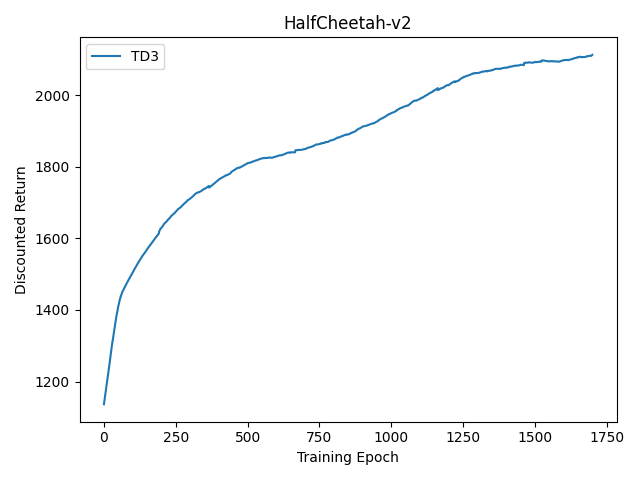
\includegraphics[scale=0.4]{figures/halfcheetah}
\caption{Discounted reward over training epoch for a TD3 agent trained on the MuJoCo HalfCheetah-v2 environment.}
\end{figure}

\begin{figure*}[!p]
\centering
  \begin{subfigure}{0.18\textwidth}
  \centering
  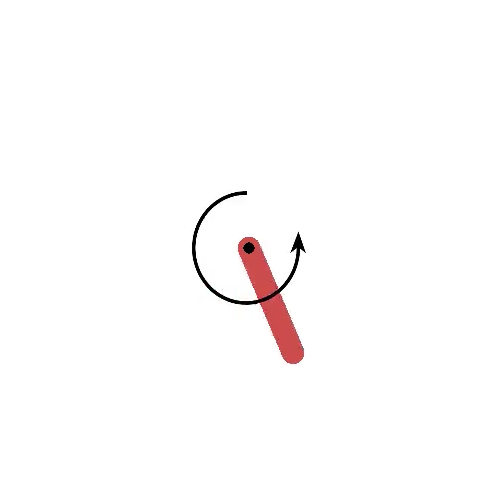
\includegraphics[width=\textwidth]{figures/pendulum/f1}
  \caption{}
  \end{subfigure}
  \begin{subfigure}{0.18\textwidth}
  \centering
  
\includegraphics[width=\textwidth]{figures/pendulum/f2}
  \caption{}
  \end{subfigure}
  \begin{subfigure}{0.18\textwidth}
  \centering
  
\includegraphics[width=\textwidth]{figures/pendulum/f3}
  \caption{}
  \end{subfigure}
  \begin{subfigure}{0.18\textwidth}
  \centering
  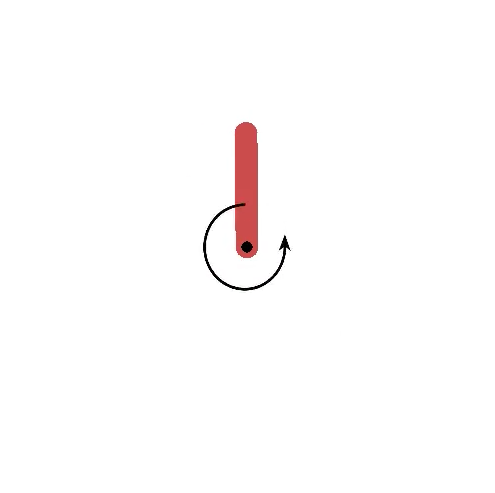
\includegraphics[width=\textwidth]{figures/pendulum/f4}
  \caption{}
  \end{subfigure}
  \begin{subfigure}{0.18\textwidth}
  \centering
  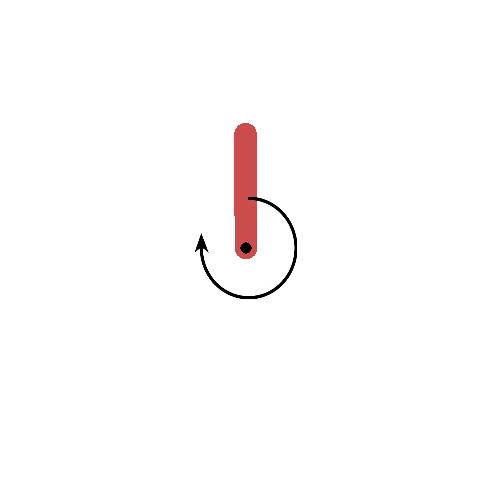
\includegraphics[width=\textwidth]{figures/pendulum/f5}
  \caption{}
  \end{subfigure}
  \caption{Sample episode of TD3 agent simulated on the Pendulum-v0 environment. The obtain the most reward, the agent must first spin the inverted pendulum up so it is balanced, and then maintain the balance for the remainder of the episode.In the sample episode, the agent quickly spings the pendulum up to vertical, (a) and (b), and then maintains vertical orientation through a series of constant control outputs, (c), (d), (e).}
  \label{fig:pendulum_episode}
\end{figure*}


\begin{figure*}[!p]
\centering
  \begin{subfigure}{0.18\textwidth}
  \centering
  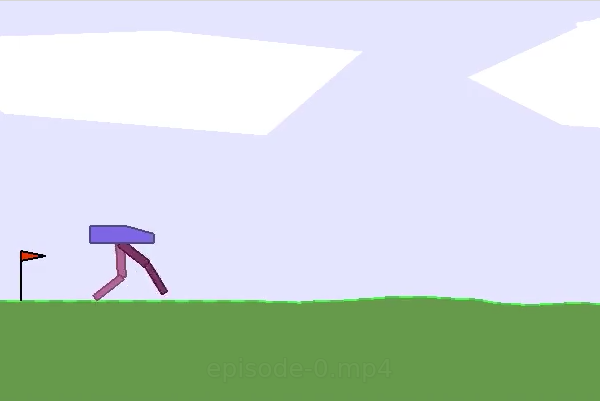
\includegraphics[width=\textwidth]{figures/bipedal/f1}
  \caption{}
  \end{subfigure}
  \begin{subfigure}{0.18\textwidth}
  \centering
  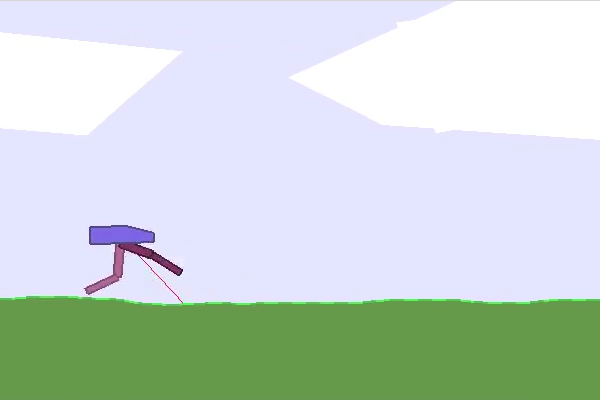
\includegraphics[width=\textwidth]{figures/bipedal/f2}
  \caption{}
  \end{subfigure}
  \begin{subfigure}{0.18\textwidth}
  \centering
  
\includegraphics[width=\textwidth]{figures/bipedal/f3}
  \caption{}
  \end{subfigure}
  \begin{subfigure}{0.18\textwidth}
  \centering
  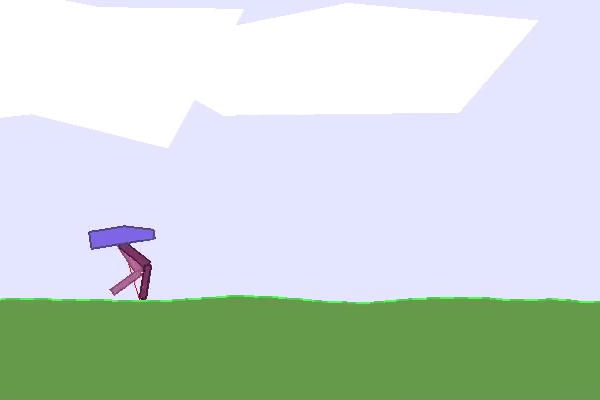
\includegraphics[width=\textwidth]{figures/bipedal/f4}
  \caption{}
  \end{subfigure}
  \begin{subfigure}{0.18\textwidth}
  \centering
  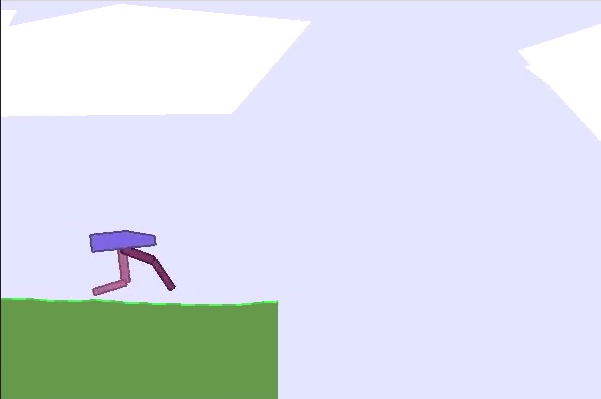
\includegraphics[width=\textwidth]{figures/bipedal/f5}
  \caption{}
  \end{subfigure}
  \caption{Sample episode of TD3 agent simulated on the BipedalWalker-v3 environment. The bipedal walker is tasked to walk for as long as possible until reaching the end of the environment despite shifts in the terrain. The walker easily reaches the end (e) under the TD3-generated policy. The red line extending from the robot indicates lidar readings that form the observation signal for the environment.}
  \label{fig:bipedal_episode}
\end{figure*}



\begin{figure*}[!p]
\centering
  \begin{subfigure}{0.18\textwidth}
  \centering
  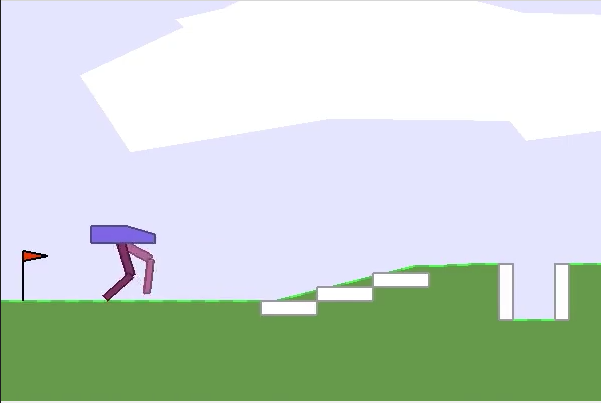
\includegraphics[width=\textwidth]{figures/hardcore/v1}
  \caption{}
  \end{subfigure}
  \begin{subfigure}{0.18\textwidth}
  \centering
  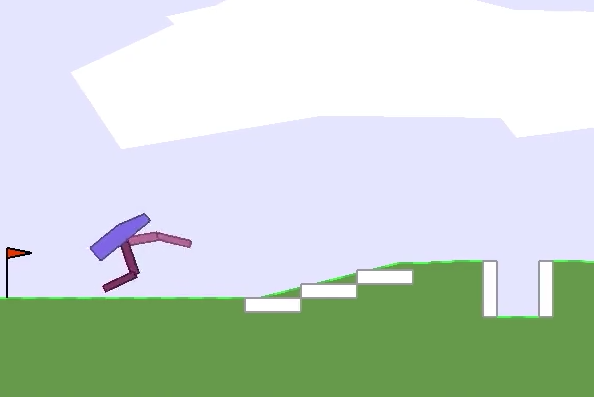
\includegraphics[width=\textwidth]{figures/hardcore/v2}
  \caption{}
  \end{subfigure}
  \begin{subfigure}{0.18\textwidth}
  \centering
  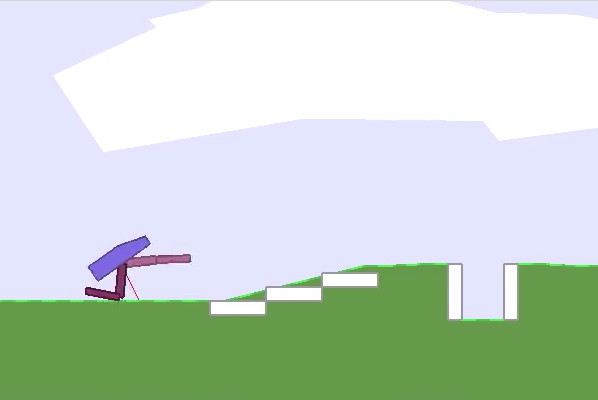
\includegraphics[width=\textwidth]{figures/hardcore/v3}
  \caption{}
  \end{subfigure}
  \begin{subfigure}{0.18\textwidth}
  \centering
  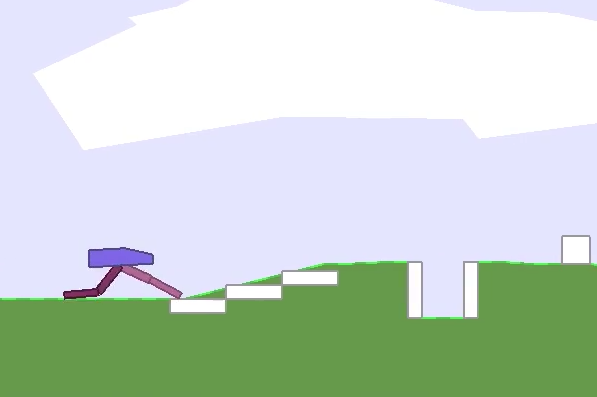
\includegraphics[width=\textwidth]{figures/hardcore/v4}
  \caption{}
  \end{subfigure}
  \begin{subfigure}{0.18\textwidth}
  \centering
  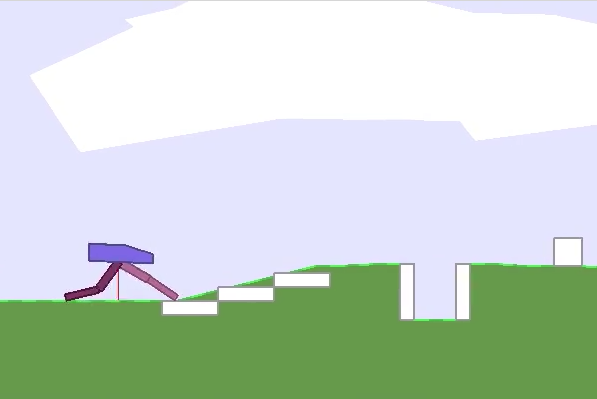
\includegraphics[width=\textwidth]{figures/hardcore/v5}
  \caption{}
  \end{subfigure}
  \caption{Sample episode of TD3 agent simulated on the BipedalWalkerHardcore-v3 environment. During training, the agent was never able to reach a successful policy, and immediately fails the sample episode. A small amount of forward progress is made, but progress immediately halts upon reaching the first obstacle (d), and remains at this point for the remainder of the episode (e).}
  \label{fig:hardcore_episode}
\end{figure*}


\begin{figure*}[!p]
\centering
  \begin{subfigure}{0.18\textwidth}
  \centering
  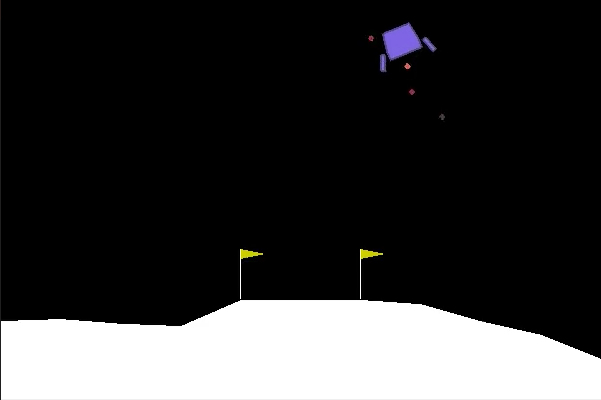
\includegraphics[width=\textwidth]{figures/lander/frame1}
  \caption{}
  \end{subfigure}
  \begin{subfigure}{0.18\textwidth}
  \centering
  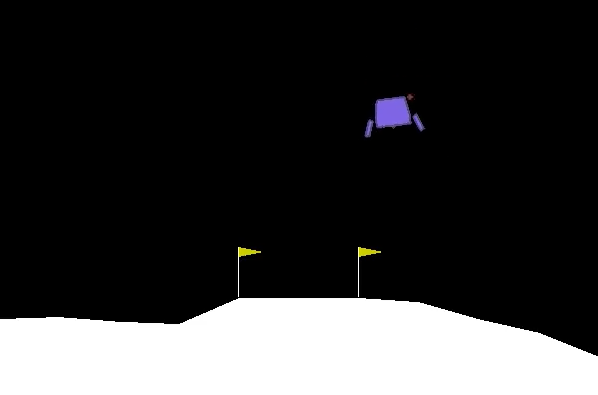
\includegraphics[width=\textwidth]{figures/lander/frame2}
  \caption{}
  \end{subfigure}
  \begin{subfigure}{0.18\textwidth}
  \centering
  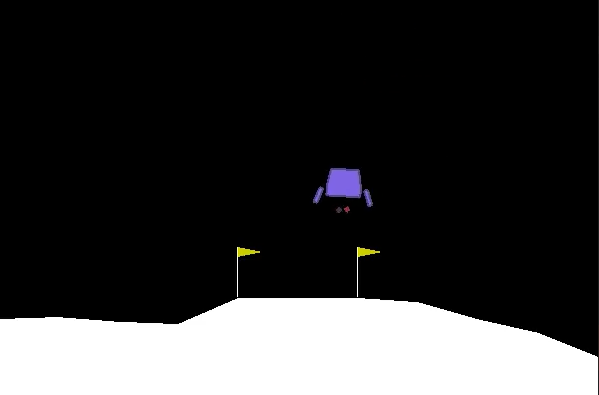
\includegraphics[width=\textwidth]{figures/lander/frame3}
  \caption{}
  \end{subfigure}
  \begin{subfigure}{0.18\textwidth}
  \centering
  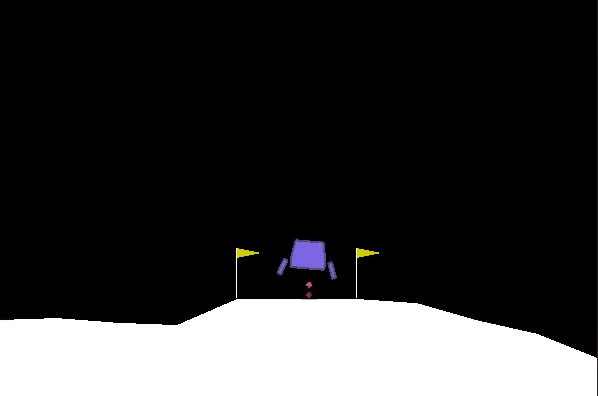
\includegraphics[width=\textwidth]{figures/lander/frame4}
  \caption{}
  \end{subfigure}
  \begin{subfigure}{0.18\textwidth}
  \centering
  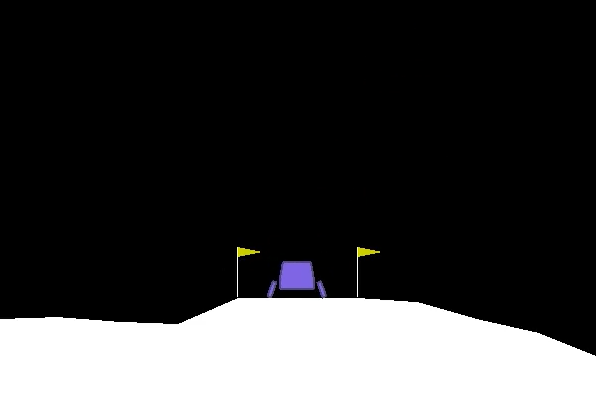
\includegraphics[width=\textwidth]{figures/lander/frame5}
  \caption{}
  \end{subfigure}
  \caption{Sample episode of TD3 agent simulated on the LunarLanderContinuous-v2 environment. The lander initially is poised to miss the target landing area (a). By effectively actuating thrusters governed by the TD3-genterated policy (b),(c),(d), the agent successfully reaches the landing zone (e)}
  \label{fig:lander_episode}
\end{figure*}


These initial experiments reveal several notable results. First and foremost, both TD3 and DDPG increase their reward over time, indicating that my implementation is functioning correctly since learning clearly occurs. On the most simple problem (the pendulum), DDPG and TD3 produce comparable results, indicating that the TD3 improvements are less pronounced on simpler tasks. Next, TD3 outperforms DDPG on the Lunar Lander problem, and dramatically outperforms DDPG on BipedalWalker, revealing the benefits gained from the TD3 improvements. Finally, while TD3 does perofrm better than DDPG on BipedalWalkerHardcore, both fail to produce an agent that accrues positive reward. I would speculate that this task may be possible with a TD3 approach, but clearly needs different hyper-parameters, training time, and/or network configurations. Note that these specific environments are not benchmarked in the original paper or the code source. Both of these sources favor MuJoCo environments for benchmarks, 

While I couldn't run large-scale MuJoCo environment tests, I was able to train an agent locally on a MuJoCo environment to compare with the original TD3 paper \cite{td3}. A perfect one-to-one comparison is not possible for several reasons. First, the original papers formulates their reward plots as time steps vs. average return, while mine plots a running average over training epoch (this stems from the difference between the runner script formulation). Furthermore, due to updates in MoJoCo, my agent trained on HalfCheetah-v2 as opposed to HalfCheetah-v1. While results should be consistent between the environments, internal changes to MuJoCo could affect results. Finally, due to time and computational limitations, I was not able to train for as long as the original authors. nor was I able to tune hyper-parameters in the same manor. These comparison limitations aside, several observations can be made. First, the reward curve is smooth and follows a similar shape as the benchmark in \cite{td3}. While I cannot say for certain that they perform the same, it does seem apparent that both learn to perform the given task, and indicates that my implementation is functional.


\FloatBarrier
\bibliography{references}
\bibliographystyle{icml2020}



\end{document}
